\chapter{TLMManager System Design}
The TLMManager is responsible for managing the TLM based co-simulation. 
The main component used in the TLMManager is an instance of {\em ManagerCommHandler} that takes a composite model as input.
{\scriptsize
\begin{verbatim}
    //! Constructor.
    ManagerCommHandler(MetaModel& Model):
        MessageQueue(),
        Comm(Model.GetComponentsNum(), Model.GetSimParams().GetPort()),
        TheModel(Model),
        CommMode(CoSimulationMode),
        monitorInterfaceMap(),
        monitorMapLock(),
        runningMode(StartUpMode)
    {
    };
\end{verbatim}
}

A {\em MetaModel} instance can be generated in different ways. 
The default TLM co-simulation implementation contains an XML composite model reader, see also Figure~\ref{fig:MetaModelReader}. 
For details about the XML composite model description see Section~\ref{meta}.

\begin{figure}[ht]
\begin{center}
  {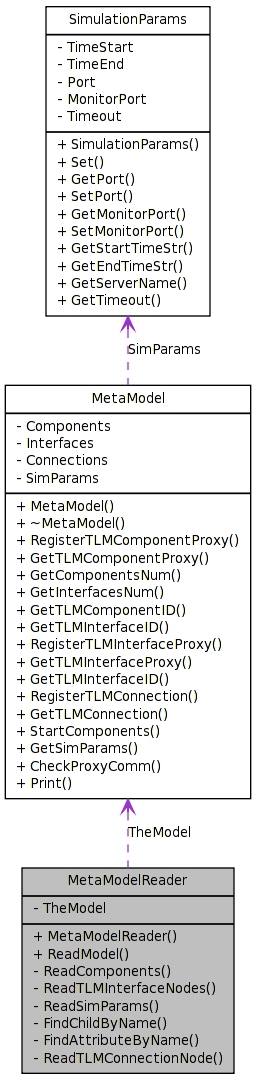
\includegraphics[width=4cm]{figs/classMetaModelReader__coll__graph.png}}
\end{center}
\caption{UML collaboration diagram of the MetaModelReader class. The
  MetaModel reader initialized the MetaModel data structure.}
\label{fig:MetaModelReader}
\end{figure}

The {\em MetaModelReader} parses the XML composite model file and initializes {\em MetaModel} and {\em SimulationParams} data structures, that is, set-up co-simulation parameters. 
Simulation parameters define global co-simulation settings, e.g., start and end time. 
Composite model parameters define the co-simulation components (simulation models) and their interconnection.

The {\em ManagerCommHandler} is then started, that is, the {\em Run()} function is invoked. 
This function initialized the different threads that are used during the co-simulation:
{\scriptsize
\begin{verbatim}
// Run method executes all the protocols in the right order:
// Startup, Check then Simulate
void ManagerCommHandler::Run(CommunicationMode CommMode_In) {
    CommMode = CommMode_In;

    pthread_attr_t attr;
    pthread_attr_init(&attr);
    pthread_attr_setscope(&attr,  PTHREAD_SCOPE_SYSTEM);
    pthread_t reader, writer;

    // start the reader & writer threads
    pthread_create( &reader, &attr, thread_ReaderThreadRun, (void*)this);

    pthread_create( &writer, &attr, thread_WriterThreadRun, (void*)this);

    // Start the minitoring thread
    pthread_t monitor;
    if( CommMode == CoSimulationMode ){
        pthread_create( &monitor, &attr, thread_MonitorThreadRun, (void*)this);
    }

    // Wait until all threads are finished.
    pthread_join(reader, NULL);
    pthread_join(writer, NULL);

    if( CommMode == CoSimulationMode ){
        pthread_join(monitor, NULL);
    }
}
\end{verbatim}
}

Note, that all communication between the co-simulation participants (simulators with models) is going through the TLM manager. 
This communication is handled by the threads that are started in the {\em Run()} function. 
The following threads are started:
\begin{description}
\item[The reader thread] initialized the co-simulation, processes incoming messages, and creates messages to be sent. 
This threads first task is to run the {\em RunStartupProtocol()} that starts all the simulation tools that are participating in the co-simulation and runs the initiation protocol. 
After that the thread goes into message passing mode. 
Messages from one co-simulation participant to another are taken by the reader thread and marshaled to the receiver, that is, they are converted into outgoing messages.
\item[The writer thread] processes all outgoing messages. 
It loops through the queue of outgoing messages and distributes them to the correct receivers.
\item[The monitor thread] copies and forwards all outgoing messages to any connected monitoring process. 
This can be used to monitor the co-simulation. 
If no monitoring process is connected no copying and forwarding will take place.
\end{description}

\begin{figure}
    \begin{center}
    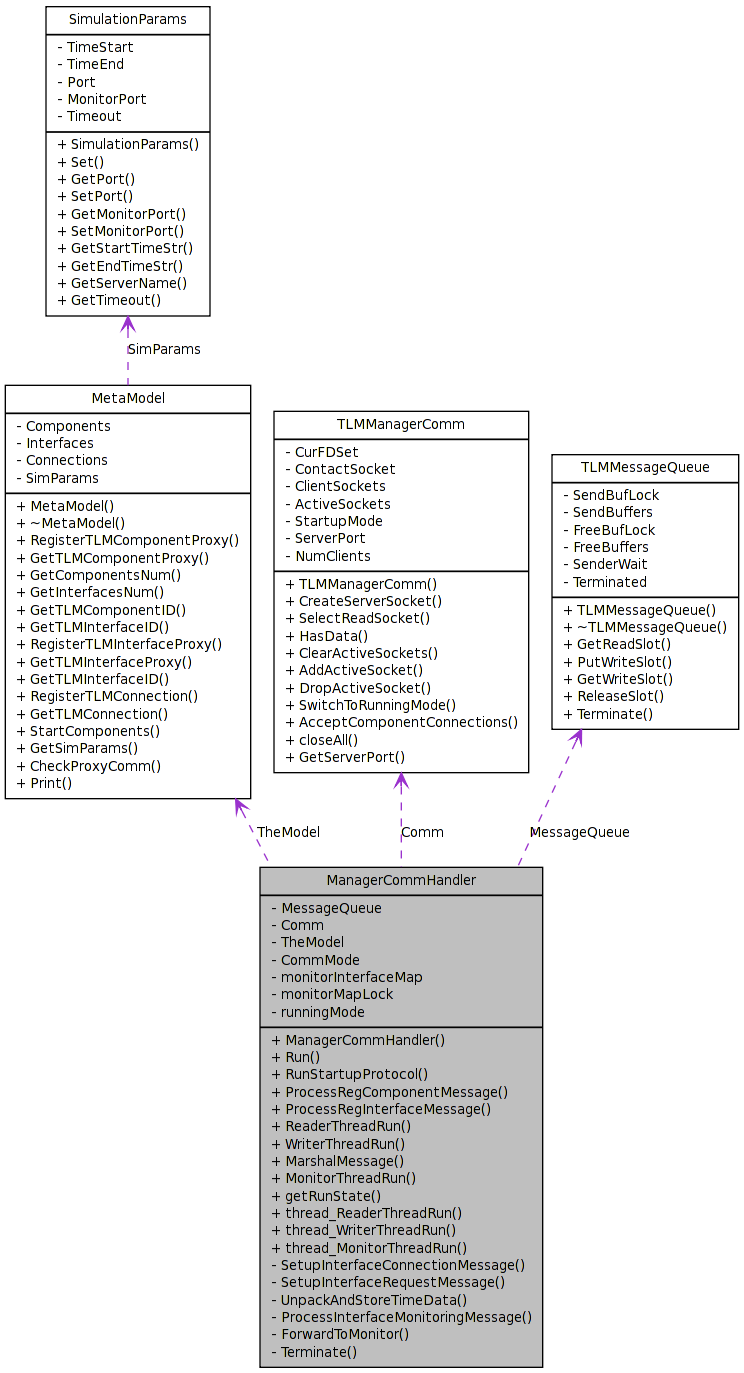
\includegraphics[width=9cm]{figs/classManagerCommHandler__coll__graph.png}
      \caption{ManagerCommHandler collaboration and class diagram.}
      \label{fig:ManagerCommHandlerClassDesign}
    \end{center}
\end{figure}

The {\em ManagerCommHandler} collaborates with different classes to handle co-simulation start-up and communication, see also Figure~\ref{fig:ManagerCommHandlerClassDesign}. 
{\em TLMManagerComm} is responsible for all socket communications on the TLMManager side. The {\em TLMMessageQueue} handles the queue for outgoing messages.

\subsection{Co-Simulation Start-up}
During co-simulation start-up the TLMManager starts the different co-simulation components (external models) and then waits until all components have registered themselves. 
This is done with a simple initialization protocol.

First the components are started using {\tt TLMComponentProxy::StartComponent(...)}. 
This is done using the OS specific execution method, for instance, with {\it fork()} and {\it execlp(...)} on Linux:
{\scriptsize
\begin{verbatim}
  execlp( StartCommand.c_str(), StartCommand.c_str(),
          Name.c_str(),
          startTime.c_str(),
          endTime.c_str(),
          strMaxStep.c_str(),
          serverName.c_str(),
          ModelName.c_str(),
          NULL );
\end{verbatim}
}

The start command is the start-up script that must be provided for each specific simulation tool. 
It takes a couple of parameters as specified in the composite model XML file:
\begin{description}
\item[Name] of the component as specified in the composite model XML file.
\item[Start time] of the simulation in seconds, typically 0.
\item[End time] of the simulation in seconds.
\item[Max step] for the solver to take. This is a limit set by the TLM interfaces of the specific component. 
The solver is not allowed to take larger steps.
\item[Server name] is typically the hostname or IP address that the TLMManager is running on and the port number that it is using. 
For  instance {\it 163.157.1.23:1111}.
\item[Model name] of the simulation model. Typically the input file
  needed to start the external model simulation.
\end{description}

\subsection{External Model Initialization}
After external model start-up, the TLMManager waits until all external models have registered themselves. 
This is performed in {\em ManagerCommHandler::RunStartupProtocol()}. 
Here an outline of the code:
{\scriptsize
\begin{verbatim}
void ManagerCommHandler::RunStartupProtocol() {
    ...
    // Start the external components forming "coupled simulation"
    TheModel.StartComponents();

    // Setup timer
    tTM_Info tInfo;
    TM_Init(&tInfo);
    TM_Start(&tInfo);

    while( (numToRegister > 0) ||
           ( numCheckModel < TheModel.GetComponentsNum()) ) {
        ...

        // Check all the registered components if they send
        // interface registration messages.
        for(int iSock =  TheModel.GetComponentsNum() - 1; iSock >= 0 ; --iSock) {
            ...
            TLMMessage* message = MessageQueue.GetReadSlot();
            message->SocketHandle = hdl;
            TLMCommUtil::ReceiveMessage(*message);

            if(message->Header.MessageType == TLMMessageTypeConst::TLM_CHECK_MODEL) {
                // This component is done with registration. It's will wait for others
                TLMErrorLog::Log(string("Component ") + comp.GetName() + " is ready to simulation");;

                comp.SetReadyToSim();
                numCheckModel++;
            }
            else {
                TLMErrorLog::Log(string("Component ") + comp.GetName() + " registers interface");;

                Comm.AddActiveSocket(hdl); // expect more messages
                ProcessRegInterfaceMessage(iSock, *message);
                MessageQueue.PutWriteSlot(message);
            }
        }

        // Check if a new connection is waiting to be accepted.
        if((numToRegister > 0) && Comm.HasData(acceptSocket)) {
            int hdl = Comm.AcceptComponentConnections();
            TLMMessage* message = MessageQueue.GetReadSlot();
            message->SocketHandle = hdl;

            if( !TLMCommUtil::ReceiveMessage(*message) ){
                TLMErrorLog::FatalError("Failed to get message, exiting");
                abort();
            }

            ProcessRegComponentMessage(*message);

            MessageQueue.PutWriteSlot(message);
            numToRegister --;
            if(numToRegister == 0)
                TLMErrorLog::Log("All expected components are registered");

            Comm.AddActiveSocket(hdl);
        }

        if(numToRegister)  // still more connections expected
            Comm.AddActiveSocket(acceptSocket);

    }
}
\end{verbatim}
}
The above method has two main tasks, first to check for new connections from any external model. 
Second to check if already registered components need to register any TLM interfaces.

The initialization protocol looks the following way:
\begin{enumerate}
\item An external model send a TLMMessageTypeConst::TLM\_REG\_COMPONENT message to the TLMManager.
\item The TLMManager answers with the same message but also sets the data size of the message to 0.
\item The external model send an interface registration message (TLMMessageTypeConst::TLM\_REG\_INTERFACE).
\item The manager answers with the same message head and adds the connection parameters as stored in the composite model XML file to the data section of the message.
\item The external model repeats the interface registration for all its external (TLM) interfaces.
\item Finally the external model sends a TLMMessageTypeConst::TLM\_CHECK\_MODEL that tells that it is ready to simulate.
\item The TLMManager puts the component into {\em ready for simulation} mode.
\end{enumerate}

